% Main chapter title
\chapter{Mathematische Grundlagen}

% Chapter label
\label{fundamentals}

In diesem Kapitel werden wir die wichtigsten mathematischen Grundlagen, die wir für die Formulierung der dünnbesetzten Hauptkomponentenanalyse benötigen, einführen. 



%----------------------------------------------------------------------------------------
%	Lineare Algebra
%----------------------------------------------------------------------------------------



\section{Lineare Algebra}

Ein Großteil der Mathematik der Hauptkomponentenanalyse beruht auf Methoden der linearen Algebra. Daher werden wir im Folgendem die wichtigsten Begriffe einführen. Aufgrund des Anwendungsfalls werden wir uns hier auf reelle Vektorräume beschränken.
Zunächst Orthogonalität, dann Matrixzerlegungen, dann noch einige weitere Eigenschaften und Theoreme, die wir später benötigen.

\subsection{Orthogonalität}
\begin{defn}[Skalarprodukt \cite{jaenich}]
Sei $V$ ein reeller Vektorraum. Ein \textit{Skalarprodukt} in $V$ ist eine Abbildung $\inner{\cdot}{\cdot}: V \times V \longrightarrow \mathbb{R}$ mit den folgenden Eigenschaften:
\begin{enumerate}[(i)]
\item Für jedes $x \in V$ sind die Abbildungen
\begin{align*}
\inner{\cdot}{x}: V & \longrightarrow \mathbb{R} & \inner{x}{\cdot}: V & \longrightarrow \mathbb{R}\\
v & \longmapsto \inner{v}{x} & v & \longmapsto \inner{x}{v}
\end{align*}
linear. $\quad$ (Bilinearität)
\item $\inner{x}{y} = \inner{y}{x}$ für alle  $x,y \in V \quad$ (Symmetrie)
\item $\inner{x}{x} > 0$ für alle $x \neq 0 \quad$ (Positive Definitheit)
\end{enumerate}
\end{defn}

Allgemein versteht man unter einem \textit{euklidischem Vektorraum} ein Paar $(V, \inner{\cdot}{\cdot})$, welches aus einem reellem Vektorraum $V$ und einem Skalarprodukt $\inner{\cdot}{\cdot}$ auf $V$ besteht. Durch das Skalarprodukt wird eine Norm auf $V$ induziert:
$$\norm{v} \defeq \sqrt{\inner{v}{v}}$$
In den folgenden Kapiteln werden wir uns vor allem mit dem \textit{Standardskalarprodukt} in $\mathbb{R}^n$ beschäftigen. Dies ist gegeben durch 
$$\inner{x}{y} = x_1y_1 + \cdots + x_ny_n.$$
Die dazugehörige Norm ist die \textit{euklidische Norm} oder $l_2$-Norm, welche wir bereits zuvor in \ref{norm} gesehen haben.

\begin{defn}[Orthogonalität \cite{jaenich}]
Zwei Elemente $v,w$ eines euklidischen Vektorraums $V$ heißen \textit{orthogonal} (geschrieben $v \perp w$) wenn ihr Skalarprodukt null ist, d.h.
$$v \perp w \iff \inner{v}{w} = 0.$$
Eine Familie $(v_1, \ldots, v_n)$ in $V$ heißt \textit{orthogonal} oder \textit{Orthogonalsystem}, wenn
$$v_i \perp v_j \quad \text{für alle} \quad i \neq j.$$
Gilt zusätzlich $\inner{v_i}{v_i} = 1$ für alle $1 \leq i \leq n$, so spricht man von einem \textit{Orthonormalsystem}.
\end{defn}

\begin{defn}[Orthonormalbasis \cite{fischer}]
Sei $\inner{\cdot}{\cdot}: V \times V \longrightarrow \mathbb{R}$ ein Skalarprodukt. Ein System von Vektoren $(v_1, \ldots, v_n)$ in $V$ wird als \textit{Orthogonalbasis} (bzw. \textit{Orthonormalbasis}) bezeichnet, wenn folgende Bedingungen erfüllt sind:
\begin{enumerate}[(i)]
\item $(v_1, \ldots, v_n)$ ist eine Basis von $V$
\item $(v_1, \ldots, v_n)$ ist ein Orthogonalsystem (bzw. Orthonormalsystem)
\end{enumerate}
\end{defn}

\begin{thm}[Existenz einer Orthonormalbasis (Fischer Lineare Algebra)]
Jeder endlichdimensionale euklidische Vektorraum besitzt eine Orthonormalbasis.
\end{thm}

\begin{thm}[Verallgemeinerter Satz des Pythagoras \cite{anton}]
\label{pythagoras}
Für orthogonale Vektoren $u,v$ in einem euklidischem Vektorraum $V$ gilt
$$\norm{u+v}^2 = \norm u^2 + \norm v^2.$$
\end{thm}

Der Begriff der Orthogonalität lässt sich auf Matrizen übertragen.

\begin{defn}[Orthogonale Matrix \cite{anton}]
Eine Matrix $A \in \mathbb{M}(n \times n, \mathbb{R})$ heißt 		\textit{orthogonal}, falls deren Zeilen und Spalten jeweils paarweise orthonormal sind, d.h.
$$\mat A^T \mat A = \mathbb{1}_n$$
\end{defn}

\begin{defn}[Orthogonalprojektion (Wikipedia)]
Eine \textit{Orthogonalprojektion} auf einen Untervektorraum $U$ eines Vektorraums $V$ ist eine lineare Abbildung $P_U \colon V \rightarrow V$, die für alle Vektoren $v\in V$ die beiden Eigenschaften
\begin{enumerate}[(i)]
\item $P_U(v) \in U \quad$   (Projektion)
\item $\langle P_U(v) - v , u \rangle = 0$ für alle $u \in U \quad$ (Orthogonalität)
\end{enumerate}
erfüllt.
\end{defn}

Mithilfe einer Orthogonalbasis für $U$ lässt sich aus dieser Definition eine Lösung für die Orthogonalprojektion $P_U(v)$ herleiten.

\begin{thm}[\cite{anton}]
Ist $(u_1, \ldots, u_n)$ eine Orthogonalbasis von $U$, so gilt für alle $v \in V$
$$P_{U}(v) = \sum_{i=1}^n \frac{\langle v, u_i \rangle}{\langle u_i, u_i \rangle} u_i$$
\end{thm}

In späteren Kapiteln werden wir die Orthogonalprojektion in einer anderen Form nutzen. Wir können die Projektion auch als Matrix-Vektor-Produkt auffassen. Verwenden wir das Standardskalarprodukt so gilt mit einer Orthogonalbasis $(u_1, \ldots, u_n)$ von $U$:
$$P_U(v) = \sum_{i=1}^n \frac{v^T u_i}{u_i^T u_i} u_i = \sum_{i=1}^n \frac{u_i u_i^T}{u_i^T u_i}v = \mat A \mat A^T v$$
wobei die Spalten von $\mat A$ die normalisierten Vektoren der Orthogonalbasis sind, d.h. $\mat A = \begin{bmatrix} \frac{u_1}{\norm{u_1}} & \cdots & \frac{u_n}{\norm{u_n}} \end{bmatrix}$

(Von Wikipedia)
The orthonormality condition can also be dropped. If $u_{1},\ldots ,u_{k}$ is a (not necessarily orthonormal) basis, and $\mat A$ is the matrix with these vectors as columns, then the projection is:
$$P_{A}=A(A^{\mathrm{T}}A)^{-1}A^{\mathrm{T}}$$

Mithilfe von \ref{pythagoras} lässt sich zeigen, dass der orthogonal auf den Unterraum projizierte Vektor den Abstand zwischen dem Ausgangsvektor und dem Unterraum minimiert.

\begin{thm}[\cite{anton}]
Sei $U$ ein Unterraum eines euklidischen Vektorraums $V$. Dann ist $P_U(v)$ die beste Näherung von $u$ in $U$, d.h.
$$\norm{P_U(v) - v}^2 \leq \norm{u - v}^2 \quad \text{für alle } u \in U$$
\end{thm}


\subsection{Matrixzerlegungen}

In diesem Abschnitt werden wir uns mit verschiedenen Matrixzerlegungen beschäftigen. Dazu werden wir zunächst ...

\begin{defn}[Eigenwert, Eigenvektor \cite{anton}]
Sei $\mat{A} \in \rnn$. Ein von Null verschiedener Vektor $x \in \rn$ heißt \textit{Eigenvektor} von $\mat{A}$, wenn
$$\mat{A}x = \lambda x$$
für einen Skalar $\lambda \in \mathbb{R}$. Die Zahl $\lambda$ heißt \textit{Eigenwert} von $\mat{A}$.
\end{defn}

\begin{defn}[Diagonalisierbar \cite{anton}]
Eine quadratische Matrix $\mat A \in \rnn$ heißt \textit{diagonalisierbar}, wenn eine invertierbare Matrix $\mat P$ existiert, so dass $\mat{D} = \mat{P}^{-1}\mat{A}\mat{P}$ Diagonalgestalt hat.
\end{defn}

Es gibt nun viele verschiedene Kriterien, wann eine Matrix diagonalisierbar ist. Für unsere spätere Anwendung interessieren wir uns vor allem für die Frage, ob es zu einer gegebenen Matrix $\mat{A} \in \rnn$ eine orthogonale Matrix $\mat{P}$ gibt, die $\mat{A}$ diagonalisiert. Eine derartige Diagonalisierung wird auch als \textit{Hauptachsentransformation} bezeichnet. Dieser Name stammt ursprünglich aus der Theorie der Kegelschnitte. Hierbei ist eine Hauptachsentransformation eine orthogonale Abbildung, welche die Koordinatenachsen in die Richtungen der beiden \textit{Hauptachsen} überführt. Wir wollen uns aber vorerst nicht mit dieser geometrischen Interpretation beschäftigen, sondern mit einem mathematisch äquivalenten, in den Anwendungen aber wichtigeren Problem.

\begin{thm}[Hauptachsentransformation \cite{jaenich}]
Ist $\mat{A} \in \rnn$ eine symmetrische Matrix, so gibt es eine orthogonale Transformation $\mat{P}$, welche $\mat{A}$ in eine Diagonalmatrix $\mat{D} \defeq \mat{P}^{-1}\mat{A}\mat{P}$ der Gestalt
$$\mat{D} = \begin{bmatrix}
    \lambda_{1} & & & & & & \\
    & \ddots & & & & & \\
    & & \lambda_1 & & & & \\
    & & & \ddots & & & \\
    & & & &\lambda_r & & \\
    & & & & & \ddots & \\
    & & & & & & \lambda_{r}
  \end{bmatrix}$$
überführt. Hierbei sind $\lambda_1, \ldots, \lambda_r$ die verschiedenen Eigenwerte von $\mat{A}$.
\end{thm}

Wir können also eine symmetrische Matrix $\mat{A}$ zerlegen in $\mat A = \mat P \mat D \mat P^T$. Man kann $\mat{P}$ so konstruieren, dass die Spalten genau den Eigenvektoren von $\mat{A}$ entsprechen. Wir werden diese Umformung in späteren Kapiteln unter dem Begriff \textit{Eigenwertzerlegung} (Englisch: Eigenvalue Decomposition) verwenden. 

Eine eng verwandte, aber vielseitigere Faktorisierung von Matrizen ist die \textit{Singulärwertzerlegung}. Sie ermöglicht eine Zerlegung auch von nicht quadratischen oder nicht symmetrischen Matrizen.

\begin{thm}[Singulärwertzerlegung \cite{schaback}]
Jede Matrix $\mat{A} \in \rmn$ besitzt eine \textit{Singulärwertzerlegung} 
$$\mat{A} = \mat{U}\mat{D}\mat{V}^{T}$$
mit orthogonalen Matrizen $\mat U \in \mathbb{R}^{m \times m}$ und $\mat V \in \rnn$, sowie der Diagonalmatrix $\mat{D} = (\sigma_j\delta_{ij}) \in \rmn$.
\end{thm}

\begin{defn}[Singulärwert]
Die positiven Diagonaleinträge $\sigma_{i} > 0$ von $\mat D$ werden \textit{Singulärwerte} genannt.
\end{defn}

Nach Konvention werden die Singulärwerte von $\mat D$ absteigend sortiert, d.h. $\sigma _{1} \geq \cdots \geq \sigma _{r}$. Außerdem sind die Singulärwerte eindeutig bestimmt und stehen durch $\sigma_i = \sqrt{\lambda_i}$ in einer engen Beziehung mit den Eigenwerten $\lambda_i$ von $\mat A$. Geometrisch bedeutet diese Faktorisierung, dass sich die Matrix $A$ in zwei Drehungen $\mat U, \mat V$ und eine Streckung unterteilen lässt. Dabei korrespondieren die Streckungsfaktoren mit den Einträgen der Diagonalmatrix $\mat D$.


\subsection{Matrix Approximation}

Das Konzept von Normen lässt sich auch auf Matrizen übertragen. In späteren Kapiteln werden wir vor allem Gebrauch folgender Norm machen.

\begin{defn}[Frobeniusnorm \cite{schaback}]
Für eine Matrix $A \in \rmn$ ist die \textit{Frobeniusnorm} definiert durch
$$\norm{\mat A}_F = \left( \sum_{i=1}^{m} \sum_{j=1}^{n} \lvert a_{ij} \rvert ^{2} \right) ^{\frac{1}{2}}.$$
\end{defn}

Man zeigt leicht, dass $\norm{\mat A}_F^2 = \spur{\mat A^T \mat A}$ gilt.
Eine weitere wichtige Eigenschaft von Matrizen ist der \textit{Rang}.

\begin{defn}[Rang \cite{anton}]
Die Dimension des Zeilen- und des Spaltenraumes einer Matrix $\mat A$ heißt \textit{Rang} von $\mat A$ und wird mit $\rang{\mat A}$ bezeichnet.
\end{defn}

Später werden wir eine Matrix $\mat A$ durch eine andere, simplere Matrix $\widehat{\mat A}$ mit niedrigerem Rang approximieren. Dieses Problem ist unter dem Namen \textit{low rank approximation} im Englischen bekannt.
Mithilfe der Singulärwertzerlegung können wir eine explizite Lösung für dieses Problem angeben.

\begin{thm}[Eckart-Young-Mirsky-Theorem \cite{eckart}]
Sei
$$\mat{A} = \mat{U}\mat{D} \mat{V}^{\top} \in \mathbb{R}^{m\times n}, \quad m \leq n$$

die Singulärwertzerlegung von $\mat{A}$ und partitioniere $\mat{U}, \mat{D}$ und $\mat{V}$ wie folgt:

$$\mat{U} =: \begin{bmatrix} \mat{U}_1 & \mat{U}_2\end{bmatrix}, \quad 
\mat{D} =: \begin{bmatrix} \mat{D}_1 & 0 \\ 0 & \mat{D}_2 \end{bmatrix},\quad \mat{V} =: \begin{bmatrix} \mat{V}_1 & \mat{V}_2 \end{bmatrix},$$

wobei $\mat{U}_{1} \in \mathbb{R}^{m\times r}$, $\mat{D} _{1} \in \mathbb{R}^{r\times r}$ und $\mat{V}_{1} \in \mathbb{R}^{n\times r}$. Dann löst die abgeschnittene Singulärwertzerlegung (Englisch: \textit{truncated singular value decomposition)}

$$\widehat \mat{A}^* = \mat{U}_1 \mat{D}_1 \mat{V}_1^{\top},$$

das Approximationsproblem

$$\min_{\operatorname{rank}(\widehat \mat{A}) \leq r} \|\mat{A}-\widehat \mat{A}\|_{\text{F}} = \|\mat{A}-\widehat \mat{A}^*\|_{\text{F}} = \sqrt{\sigma^2_{r+1} + \cdots + \sigma^2_m},$$

wobei $\sigma_i$ die Singulärwerte von $\mat A$ bzw. die Diagonaleinträge von $\mat D$ sind. Der Minimierer $\widehat \mat{A}^*$ ist genau dann eindeutig, wenn $\sigma_{r+1} \neq \sigma_{r}$.
\end{thm}

Ein weiteres Problem, was unter diese Kategorie fällt ist Procrustes Rotationsproblem.

\begin{thm}[Procrustes Rotationsproblem \cite{gower}]
Seien $\mat M \in \mathbb{R}^{n \times p}$, $\mat N \in \mathbb{R}^{n \times k}$ und $\mat M^T \mat N = \mat{U}\mat{D} \mat{V}^{\top}$ eine Singulärwertzerlegung. Dann löst
$$\hat{\mat A} = \mat U \mat V^T$$
das Approximationsproblem
$$\hat{\mat A} = \argmin_{\mat A} \norm{\mat M - \mat N \mat A^T}_F^2$$
$$\text{unter der Nebenbedingung, dass } \mat A^T \mat A = \mat I_{k \times k}.$$
\end{thm}


%----------------------------------------------------------------------------------------
%	Analysis
%----------------------------------------------------------------------------------------


\section{Analysis}

In diesem Abschnitt möchten wir die 

\subsection{Norm}

\begin{defn}[\cite{hieber}]
\label{norm}
Eine Abbildung $\norm{\cdot} \colon \mathbb{R}^n \longrightarrow {\mathbb {R} }_{0}^{+}$ heißt \textit{Norm}, falls für alle Vektoren $x,y\in \mathbb{R}^n$ und alle Skalare $\alpha \in \mathbb{R}$ die folgenden drei Axiome gelten:
\begin{enumerate}[(i)]
\item \makebox[4cm][l]{$\|x\|=0\;\Leftrightarrow \;x=0$}(Definitheit)
\item \makebox[4cm][l]{$\|\alpha \cdot x\|=|\alpha |\cdot \|x\|$}(Homogenität)
\item \makebox[4cm][l]{$\|x+y\|\leq \|x\|+\|y\|$}(Subadditivität)
\end{enumerate}
\end{defn}

\begin{defn}[$l_p$-Norm \cite{schaback}] 
Auf dem $\mathbb{R}^n$ sind die $l_p$-Normen für $1 \leq p < \infty$ definiert als
$$\norm{x}_p \defeq \left( \sum_{i=1}^{n} \abs{x_i}^{p} \right) ^{\frac{1}{p}} \quad x \in \mathbb{R}^{n}$$
und für $p = \infty$ als
$$\norm{x}_{\infty} \defeq \max_{1 \leq i \leq n} \abs{x_i} \quad x \in \mathbb{R}^{n}.$$
Im Fall $p = \infty$ spricht man auch von der \textit{Maximumsnorm} und im Fall $p = 2$ von der \textit{euklidischen Norm}.
\end{defn}

Eine weitere wichtige Norm, die wir im Zuge dieser Arbeit verwenden werden ist die $l_0$-\q{Norm}. Diese zählt die von null verschiedenen Einträge eines Vektors und misst somit, ob ein Vektor dünnbesetzt ist.

\begin{defn}[$l_0$-\q{Norm} \cite{foucart}]
Die sogenannte $l_0$-\q{Norm} ist definiert durch
$$\norm{x}_{0} \defeq \left|\{i \colon \enspace x_i \neq 0 , \quad 1 \leq i \leq n\}\right|.$$
\end{defn}

Die übliche Schreibweise $\norm{x}_0$ - die Notation $\norm{x}_{0}^{0}$ wäre angemessener - entspringt der Beobachtung, dass 
$$\norm{x}_{p}^{p} = \sum_{i=1}^{n} \abs{x_i}^p \quad \underset{p \rightarrow 0}{\longrightarrow} \quad \sum_{i=1}^{n} \mathbb{1}_{\{x_i = 0\}} = \left|\{i \colon \enspace x_i \neq 0\, , \quad 1 \leq i \leq n\}\right|$$
Wir wollen betonen, dass die $l_0$-\q{Norm} keine wirkliche Norm ist, da die Abbildung nicht homogen ist. Trotzdem ist diese \q{Norm} in der Theorie der komprimierten Erfassung (Englisch: \textit{compressive sensing}) sehr nützlich. (Trotzdem wird sie im Folgenden eine entscheidene Rolle spielen)

%----------------------------------------------------------------------------------------
%	Statistik
%----------------------------------------------------------------------------------------

\section{Statistik}
Varianz, Erwartungswert
bias variance trade-off (Murphy, Machine Learning)
\subsection{Empirische Kovarianzmatrix}

\subsection{Lineare Regressionsmodelle}

Es existiert eine sehr enge Verbindung zwischen der Hauptkomponentenanalyse, die wir in Kapitel \ref{pca} näher kennenlernen werden, und der Regressionsanalyse. Viele der Ideen und Ansätze im folgendem Abschnitt werden wir später gebrauchen und spielen eine maßgebliche Rolle bei der Formulierung der dünnbesetzten Hauptkomponentenanalyse.\\

\textbf{Lineare Regression} \cite{hastie_elements}

Bei der Regressionsanalyse werden Zusammenhänge zwischen
mehreren Merkmalen untersucht. Man versucht eine unabhängige Variable $Y$ durch eine oder mehrere abhängige Variablen $X_1, \ldots, X_p$ zu erklären. Ein lineares Regressionsmodell hat also die Form
\begin{align}
\label{linear_model}
f(X) = \beta_0 + \sum_{j=1}^p X_j\beta_j
\end{align}
wobei $\beta_j$ die Regressionskoeffizienten sind.
Bei der Verwendung dieses Modells nehmen wir an, dass die Regressionsfunktion $\text{E}(Y|X)$ linear ist bzw. ein lineares Modell eine geeignete Approximation ist.

Typischerweise verfügen wir über eine Menge von Trainingsdaten $(x_1, y_1), \ldots, (x_n, y_n)$. Jedes $x_i = (x_{i1}, \ldots, x_{ip})^T$ stellt eine Beobachtung dar, die wir für die Schätzung der Parameter $\beta_j$ benutzen. Die bekannteste Methode für diesen Zweck ist sicherlich die \textit{Methode der kleinsten Quadraten} (Englisch: \textit{(Ordinary) Least Squares}), in welcher wir $\beta = (\beta_0, \ldots, \beta_p)^T$ wählen, so dass die Summe der Residuenquadrate (Englisch: \textit{Residual Sum of Squares}, kurz RSS) minimiert wird. Wir definieren
\begin{align}
\label{RSS}
\text{RSS}(\beta) & = \sum_{i=1}^{n}(y_i - f(x_i))^2\\
& = \sum_{i=1}^{n}(y_i - \beta_0 - \sum_{j=1}^p x_{ij}\beta_j)^2\\
& = (y - \mat X \beta)^T(y-\mat X \beta)\\
& = \norm{y - \mat X \beta}_{2}^{2}
\end{align}
und das dazugehörige Minimierungsproblem
\begin{align}
\label{least_squares}
\hat{\beta}^{\text{OLS}} = \argmin_{\beta} \text{RSS}(\beta)
\end{align}
wobei $\mat X \in \mathbb{R}^{n \times (p+1)}$ die Matrix der $x_i$ mit einer 1 an erster Stelle ist und $y = (y_1, \ldots, y_n)^T$. Eine Visualisierung der Methode befindet sich in Abbildung REF. Vielleicht Bild zur Regression in 2 bzw. 3D?

An dieser Stelle möchten wir erwähnen, dass bei Verwendung dieser Methode keine Aussage über die Gültigkeit des Modells getroffen, sondern lediglich die beste lineare Approximation gefunden wird.

Falls $\mat X$ vollen Rang hat, ist es ist leicht zu zeigen, dass (\ref{least_squares}) die eindeutige Lösung
\begin{align}
\hat{\beta}^{\text{OLS}} = (\mat X^T\mat X)^{-1}\mat X^T y
\end{align}
besitzt. Die Zielgröße ergibt sich dann durch
\begin{align}
\hat{y} = \mat X \hat{\beta}^{\text{OLS}} = \mat X (\mat X^T\mat X)^{-1}\mat X^T y
\end{align}
Die Matrix $\mat H = \mat X (\mat X^T\mat X)^{-1}\mat X^T$ haben wir bereits in REF kennengelernt. Sie projiziert $y$ orthogonal auf den durch  die Spalten von $\mat X$ aufgespannten Unterraum. Dies ermöglicht eine geometrische Interpretation der linearen Regression.

Wenn $\mat X$ keinen vollen Rang hat, ist die Lösung von (\ref{least_squares}) nicht mehr eindeutig. Dieser Art Probleme ereignen sich häufig in der Bild- und Signalanalyse, da es mehr Variablen als Beobachtungen gibt ($p > n$). Um ein gewünschtes Verhalten der Regression zu gewährleisten, bestehen verschiedene Möglichkeiten der Filterung oder Regularisierung. In letzterem Fall versehen wir den Regressionsterm mit sog. \textit{Straftermen}. Diese werden eine bedeutende Rolle in den folgenden Kapitel spielen.

Gelegentlich sind wir mit den Ergebnissen der Methode der kleinsten Quadrate nicht zufrieden. Dies kann zum Beispiel an der Multikollinearität des Datensatzes liegen. Mit zunehmender Multikollinearität ist die Methode instabil und bei der Schätzung der Regressionskoeffizienten ungenau. Es ergeben sich die folgenden zwei Probleme:
\begin{itemize}
\item Vorhersagegenauigkeit: Meist hat das erzeugte Modell einen niedrigen Bias, aber eine hohe Varianz. Somit sind neue Vorhersagen, die wir auf zuvor ungesehenen Daten treffen, oft sehr ungenau. In manchen Fällen können wir die Ergebnisse durch eine Erhöhung des Bias verbessern, indem wir die Regressionskoeffizienten verkleinern oder sogar auf 0 setzen.
\item Interpretation: Eine hohe Anzahl an Variablen, die in das Modell einfließen erschwert unzweifelhaft eine Interpretation. Daher kann es von Vorteil sein nur den Teil der Variablen für das Modell auszuwählen, die den größten Effekt für die Vorhersage erzielen.
\end{itemize}

Ein naheliegender Ansatz zur Lösung dieser Probleme wäre es zu versuchen, die beste Teilmenge an Variablen zu finden, die eine minimale Summe der Residuenquadrate aufweist. In \cite{hastie_elements} werden verschiedene Methoden zur exakten und approximativen Berechnung dieser Teilmenge beschrieben. (Darunter fallen die leaps and bounds Methode (Furnival and Wilson, 1974), Forward Stepwise und Backward Stepwise.) Nicht immer wird die Genauigkeit der Vorhersagen durch Verwendung dieses Ansatzes besser. Dies liegt daran, dass es sich um einen diskreten Prozess handelt und somit Variablen für das Modell entweder ausgewählt oder verworfen werden. Daher beschäftigen wir uns nun mit Methoden, die eine kontinuierliche Schrumpfung der Regressionskoeffizieten erlauben.\\

\textbf{Ridge Regression}

Die \textit{Tikhonov Regularisierung}, die auch unter dem Namen \textit{Ridge Regression} bekannt ist, kann genutzt werden, um das Problem der Multikollinearität zu lösen und im Fall $p > n$ eine eindeutige Lösung zu erhalten.
Wie wir bereits in REF gesehen haben, kann es sinnvoll sein den Bias zu erhöhen, um genauere Vorhersagen treffen zu können. Daher führen wir nun eine \textit{ridge penalty}, einen Strafterm, ein und formulieren das Ridge Regression Problem in der Lagrange Form.
\begin{align}
\label{ridge_regression}
\hat{\beta}^{\text{ridge}} = \argmin_{\beta} \sum_{i=1}^{n}(y_i - \beta_0 - \sum_{j=1}^p x_{ij}\beta_j)^2 + \lambda\sum_{j=1}^p \beta_j^2
\end{align}
wobei $\lambda \geq 0$ ein Parameter ist, der die Stärke der Schrumpfung der Regressionskoeffizienten kontrolliert. Je größer $\lambda$, desto stärker ist die Schrumpfung der $\beta_j$. Man kann zeigen, dass die Lösung von (\ref{ridge_regression}) in zwei Teile aufgeteilt werden kann. Da $\beta_0$ nicht im Strafterm vorkommt, schätzen wir $\beta_0 = \bar{y} = \frac{1}{n}\sum_{i=1}^{n} y_i$ und zentrieren die Eingaben $x_{ij} = x_{ij} - \bar{x}_j$. Die eindeutige Lösung der zentrierten Version von (\ref{ridge_regression}) ist dann gegeben durch
\begin{align}
\hat{\beta}^{\text{ridge}}  = (\mat X^T \mat X + \lambda\mat{I})^{-1}\mat{X}^Ty
\end{align}
wobei $\beta = (\beta_1, \ldots, \beta_p)$ und $\mat{X} \in \mathbb{R}^{n \times p}$ die Matrix der $x_i$. (Vor der Anwendung von Ridge Regression werden die Daten meist standardisiert, da $\hat{\beta}^{\text{ridge}}$ nicht äquivariant unter Skalierung ist.) \\


\textbf{LASSO}

Die durch die Ridge Regression erzeugten Koeffizienten sind also um den Faktor $\frac{1}{1+\lambda}$ gegenüber denen von Least Squares skaliert. Die Regressionskoeffizieten werden also erst für $\lambda \rightarrow 0$ auf Null geschrumpft. Um eine bessere Interpretation des Modells zu ermöglichen kreiert das \textit{Lasso} eine dünnbesetzte Lösung, bei welcher viele Koeffizienten gleich Null sind. Das Lasso wurde erstmals von Tibshirani in \cite{tibshirani_lasso} eingeführt und ist in der Signalanalyse unter dem Namen \textit{Basis Pursuit} \cite{chen} bekannt. Mathematisch erreichen wir eine Dünnbesetzung durch Einbettung eines $l_1$-Strafterms.
\begin{align}
\label{lasso}
\hat{\beta}^{\text{lasso}} = \argmin_{\beta} \sum_{i=1}^{n}(y_i - \beta_0 - \sum_{j=1}^p x_{ij}\beta_j)^2 + \lambda\sum_{j=1}^p \left|\beta_j\right|
\end{align}
Es wird also im Vergleich zu (\ref{ridge_regression}) lediglich die $l_2$-Norm durch eine $l_1$-Norm ausgetauscht. Bevor wir uns mit der Lösung dieses Problems beschäftigen, möchten wir erklären, warum die $l_1$-Norm eine Dünnbesetzung hervorruft. Die lässt sich auf zwei Arten erklären. Zunächst geben wir eine geometrische Erklärung, welche in Abbildung REF zu sehen ist. In Abbildung REF haben wir die $l_1$- und $l_2$-Beschränkungen sowie die Höhenlinien der RSS Funktion in zwei Dimensionen aufgezeichnet. Die optimalen Koeffizienten von Ridge Regression und Lasso ergeben sich nun aus dem Schnittpunkt der Höhenlinie und der Norm-Begrenzung. Im Falle der $l_1$-Norm ist dieser Schnittpunkt mit einer hohen Wahrscheinlichkeit an eine der Ecken und einer der beiden Koeffizienten wird auf Null gesetzt. Im Gegensatz gibt es bei der Wahl einer $l_2$-Begrenzung keine Ecken. Somit kommt jeder Randpunkt der Begrenzung als Schnittpunkt in Frage und es wird keine Dünnbesetzung hervorgerufen. Dieser Effekt verstärkt sich in höheren Dimensionen.

\begin{figure}
\centering
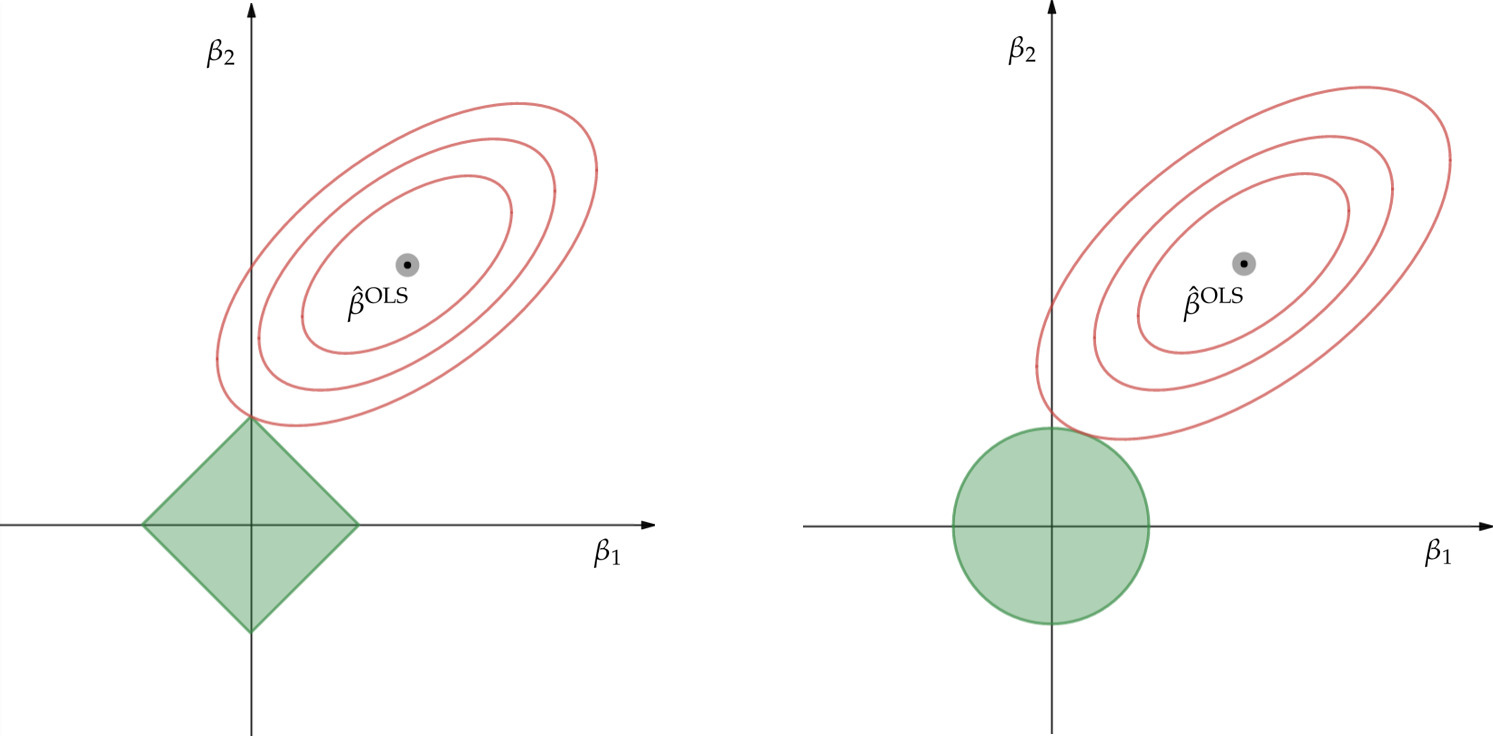
\includegraphics[width = 0.9\textwidth]{figures/lasso_ridge_regression.jpg}
\caption{Die Abbildung zeigt die Beschränkungen der $l_1$-Norm (links) und der $l_2$-Norm (rechts) zusammen mit den Höhenlinien der RSS-Funktion, welche $\hat{\beta}^{\text{OLS}}$ als Minimierer besitzt. Verdeutlicht wird hier die geometrische Findung von $\hat{\beta}^{\text{lasso}}$ (links) und $\hat{\beta}^{\text{ridge}}$ (rechts)\\Basiert auf \cite{hastie_elements}}
\label{lasso_ridge_regression_figure}
\end{figure}

Man kann durchaus auf die Idee kommen, andere Normen zu verwenden. Warum nicht $p = 0.5$ als Norm? Nochmal Plot mit verschiedenen Normen im $R^2$

\begin{figure}
\centering
	\begin{subfigure}{0.2\textwidth}
	\centering
	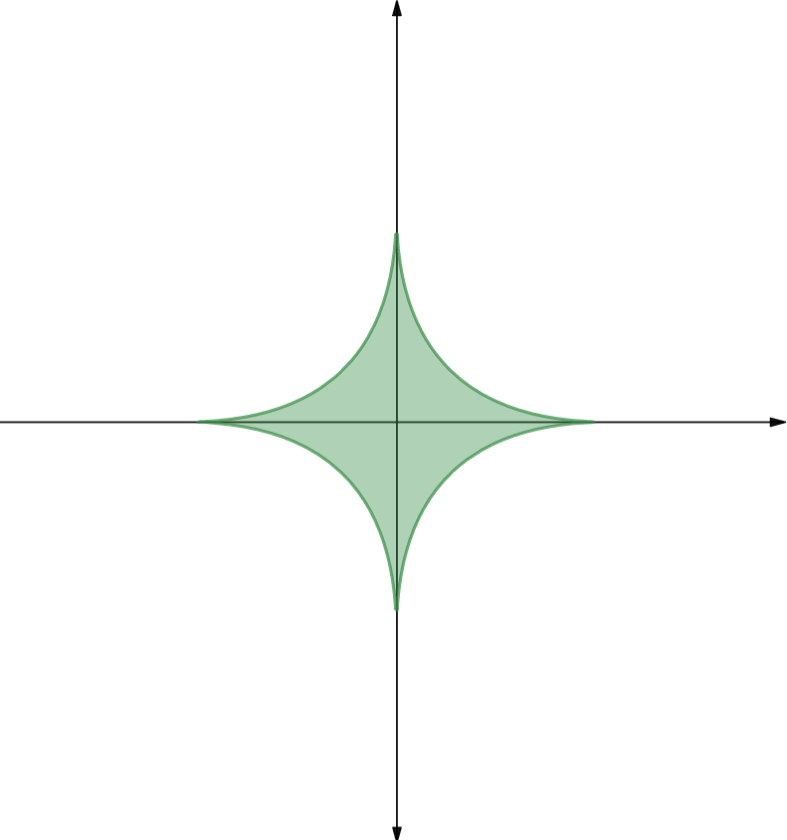
\includegraphics[width = \textwidth]{figures/norm_0_5.png}
	\label{norm_0_5_figure}
	\end{subfigure} \hspace{0.5cm}
	%	
	\begin{subfigure}{0.2\textwidth}
	\centering
	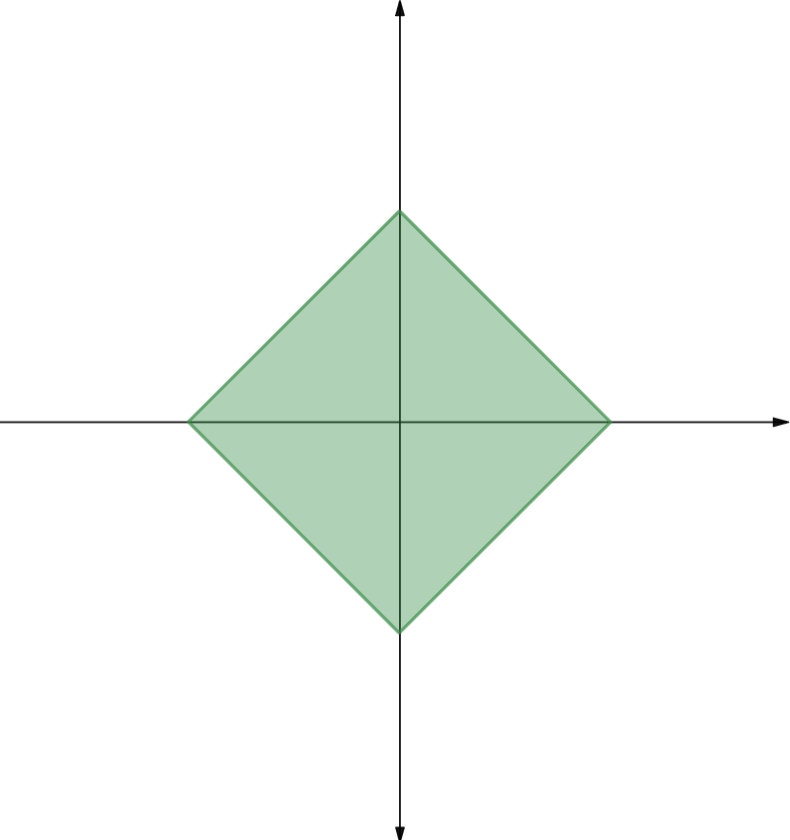
\includegraphics[width = \textwidth]{figures/norm_1.png}
	\label{norm_1_figure}
	\end{subfigure}\hspace{0.5cm}
	%
	\begin{subfigure}{0.2\textwidth}
	\centering
	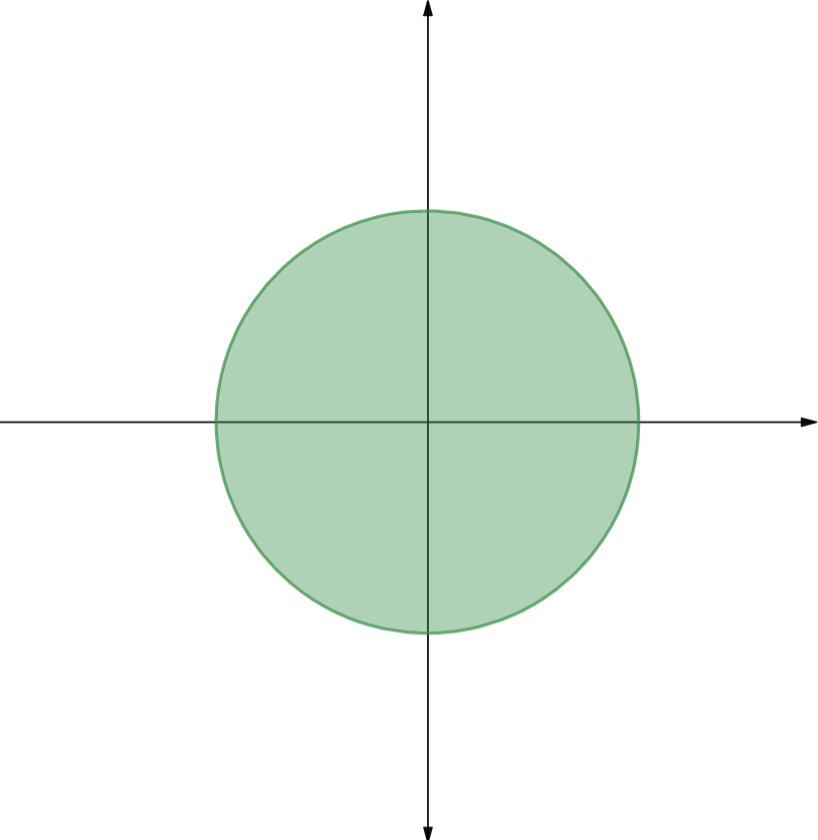
\includegraphics[width = \textwidth]{figures/norm_2.png}
	\label{norm_2_figure}
	\end{subfigure}\hspace{0.5cm}
	%
	\begin{subfigure}{0.2\textwidth}
	\centering
	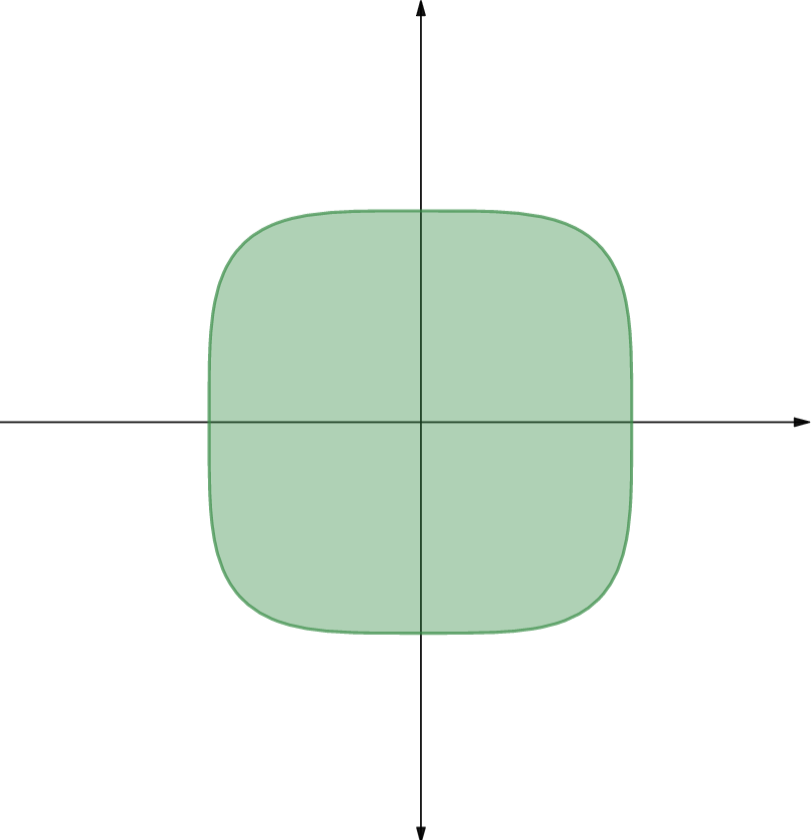
\includegraphics[width = \textwidth]{figures/norm_4.png}
	\label{norm_4_figure}
	\end{subfigure}

\caption{Die Abbildung zeigt die Normen verschiedener Größe ...}
\label{norm_figure}
\end{figure}

Um eine mathematisch gründliche Erklärung für die Dünnbesetzung zu liefern, wenden wir uns der Lösung von \ref{lasso} zu. Diese ist gegeben durch
\begin{align}
\hat{\beta}^{\text{lasso}} = \text{sign}(\hat{\beta}^{\text{OLS}}) \left(\left|\hat{\beta}^{\text{lasso}}\right| - \frac{\lambda}{2}\right)_{+}
\end{align}
Der Beweis kann in \cite{murphy} nachgelesen werden. Der sog. \textit{soft thresholding operator} $(\cdot)_+$ ist in Abbildung REF dargestellt. Warum ist dann sparsity klar? (Murphy)

\begin{figure}
\centering
	\begin{subfigure}{0.4\textwidth}
	\centering
	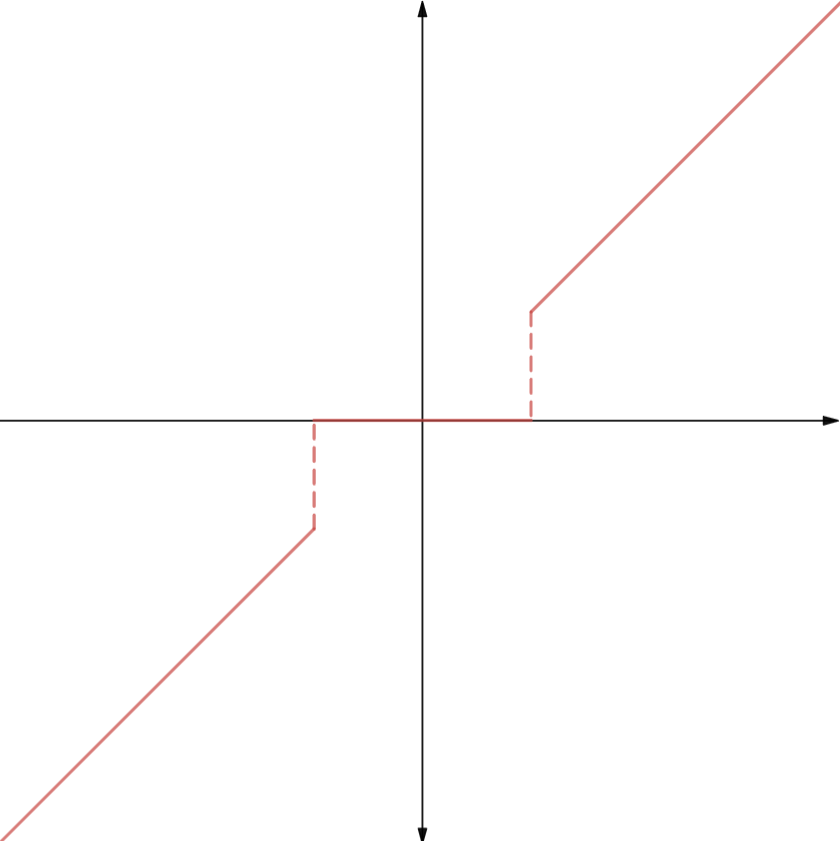
\includegraphics[width = \textwidth]{figures/hard_thresholding.png}
	\label{hard_thresholding}
	\end{subfigure}\hspace{1cm}
	%	
	\begin{subfigure}{0.4\textwidth}
	\centering
	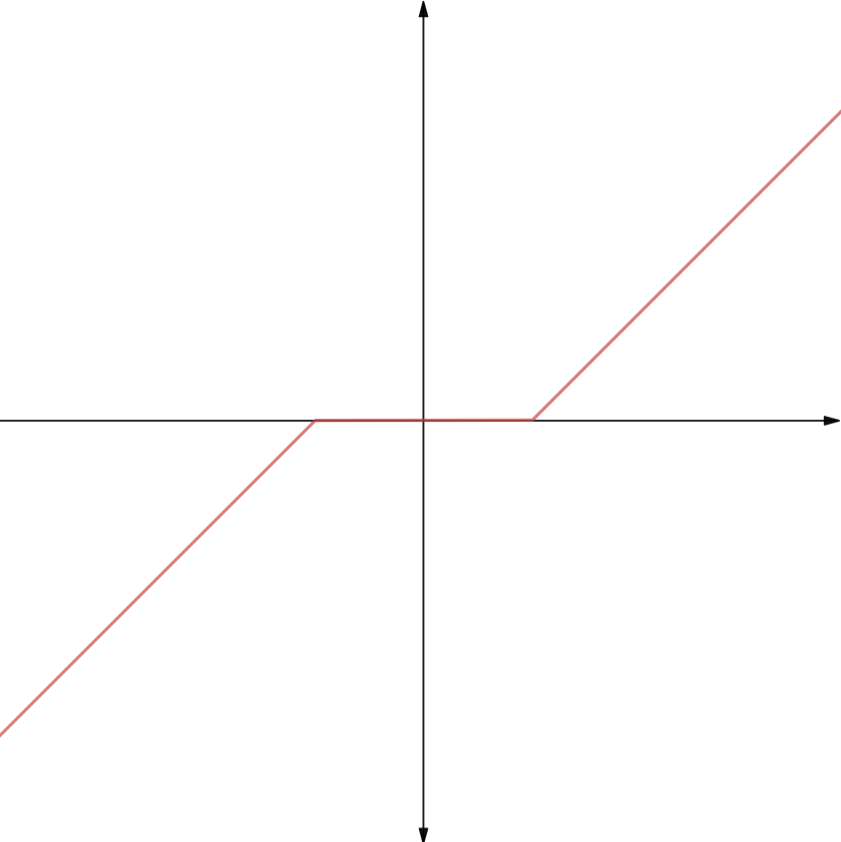
\includegraphics[width = \textwidth]{figures/soft_thresholding.png}
	\label{soft_thresholding}
	\end{subfigure}
\caption{Die Abbildung zeigt die beiden Operationen soft und hard thresholding}
\label{thresholding_figure}
\end{figure}

Mathematische Lösung des Problems? (LARS, aber nicht näher erwähnen)
plot wie Koeffizienten gegen 0\\

\textbf{Elastic Net}
Motivation warum LASSO nicht reicht. 
Mathematische Formulierung
\begin{align}
\hat{\beta}^{\text{en}} = \argmin_{\beta} \norm{y - \mat X \beta}_2^2 + \lambda \norm{\beta}_{2}^{2} + \lambda_{1,j} \norm{\beta}_{1}
\end{align}
Lösung des Problems (LARS-EN? oder hier GLM mit coordinate descent?)\\

\textbf{Vergleich der Methoden}

Zur anschaulichen Darstellung der oben eingeführten Methoden werden wir diese auf ein Beispiel anwenden. Dabei greifen wir auf einen durch scikit-learn \cite{scikit_learn} bereitgestellten Datensatz, der erstmals durch \cite{efron_lars} öffentlich gemacht worden ist, zurück. In diesem wurden für $n = 442$ Diabetes Patienten zehn verschiedene Variablen gemessen. Dazu gehören Alter (AGE), Geschlecht (SEX), Body Mass Index (BMI), Blutdruck (BP) und verschiedene Blutproben (Serum Measurements). Die Zielgröße $y$ ist eine quantitative Messung des Krankheitsfortschritts ein Jahr nach Behandlungsbeginn. Einen Überblick über den Datensatz befindet sich in Tabelle \ref{diabetes_data_set}.

\begin{table}
\centering
\begin{tabular}[c]{c|cccccccccc|c}
& \thead{AGE} & \thead{SEX} & \thead{BMI} & \thead{BP} & \multicolumn{6}{c|}{\ldots \thead{Serum Measurements} \ldots} & \thead{Response}\\
\thead{Patient} & \thead{x1} & \thead{x2} & \thead{x3} & \thead{x4} & \thead{x5} & \thead{x6} & \thead{x7} & \thead{x8} & \thead{x9} & \thead{x10} & \thead{y}\\
\hline
1 & 59 & 2 & 32.1 & 101 & 157 & 93.2 & 38 & 4 & 4.9 & 87 & 151\\
2 & 48 & 1 & 21.6 & 87 & 183 & 103.2 & 70 & 3 & 3.9 & 69 & 75\\
3 & 72 & 2 & 30.5 & 93 & 156 & 93.6 & 41 & 4 & 4.7 & 85 & 141\\
4 & 24 & 1 & 25.3 & 84 & 198 & 131.4 & 40 & 5 & 4.9 & 89 & 206\\
\vdots & \vdots & \vdots & \vdots & \vdots & \vdots & \vdots & \vdots & \vdots & \vdots & \vdots & \vdots\\
441 & 36 & 1 & 30.0 & 95 & 201 & 125.2 & 42 & 5 & 5.1 & 85 & 220\\
442 & 36 & 1 & 19.6 & 71 & 250 & 133.2 & 97 & 3 & 4.6 & 92 & 57\\
\end{tabular}
\caption{Diabetes Datensatz \cite{efron_lars, diabetes_data}}
\label{diabetes_data_set}
\end{table}


%----------------------------------------------------------------------------------------
%	Signaltheorie
%----------------------------------------------------------------------------------------


\section{Signaltheorie}

\subsection{Fouriertransformation}
\subsection{Nyquist-Shannon Abtasttheorem}

\section{Dictionary Learning}